\chapter{Analytic Forward Sensitivity Analysis}

\begin{flushright}
\textit{Differentiate the model, and the important parameters identify themselves.}
\end{flushright}

\bigskip

Chapter~3 showed how to compute sensitivity indices for any model
by finite differences. For the malaria model with 17~\POIs and
7~state variables, the centered-difference Jacobian requires
239~model evaluations, about 4~hours if each run takes a minute,
or 10~days if each takes an hour.

There is a faster and more accurate alternative, provided the model
can be differentiated analytically: differentiate the governing
equations directly. The result is a new system of equations
the \emph{forward sensitivity equations}\index{forward sensitivity equation (FSE)}, whose solution
is the exact derivative at the cost of one linear solve per \POI.
For the malaria model: 17~linear solves of a $7\times7$ system,
each taking milliseconds.

The catch is that the model must be differentiable and the
analyst must be patient enough to derive the sensitivity equations.
This chapter develops that derivation systematically,
shows that it always produces a \emph{linear} system no matter
how nonlinear the original model is, and ends by quantifying
the remaining computational bottleneck that motivates
Chapters~5 and 6.

%%------------------------------------------------------------
\section{The FSE Derivation Pattern}
\label{sec:FSEpattern}
%%------------------------------------------------------------

The forward sensitivity equation (\FSE) for any model is obtained
by a single operation: differentiate the governing equation with
respect to a \POI and apply the chain rule.
The result is always a linear equation in the sensitivity variables,
regardless of whether the original model is linear or nonlinear.

\subsection{The Pattern in Three Steps}

\textbf{Step 1.} Write the governing equation in the form
$\mathcal{F}(u; p) = 0$ or $\mathcal{F}(u; p) = f$, where $u$
is the solution and $p$ is the \POI of interest.

\textbf{Step 2.} Differentiate both sides with respect to $p$.
Apply the chain rule to every term that depends on $u$.
Collect terms. The result is an equation for $\partial u/\partial p$.

\textbf{Step 3.} Recognize that the equation from Step~2 is
\emph{linear in} $\partial u/\partial p$, even if $\mathcal{F}$
is nonlinear in $u$.

The linearity in Step~3 is not a coincidence. Differentiation is
a linear operation: applying it to a nonlinear equation in $u$
produces a linear equation in $\partial u/\partial p$.
This structural fact is what makes analytic SA computationally tractable.

\medskip
\noindent\textbf{Misconception to confront.} A common reaction to
the FSE is: ``Deriving and solving these equations must be at least
as hard as solving the original model.'' This is wrong in two ways.
First, the FSE is always \emph{linear} in the sensitivity variable,
even when the original model is highly nonlinear; a linear system
is categorically easier to solve than a nonlinear one.
Second, the FSE for an ODE uses the \emph{same} coefficient matrix
$F_u$ that the original solver already computes, so the additional
cost per parameter is one linear solve, not one full nonlinear solve.
The FSE is not a second model; it is a linear companion to the first.
\medskip

\subsection{Application to Three Model Types}

The same three-step pattern applies to algebraic systems,
difference equations, and ordinary differential equations.
Sections~\ref{sec:algebraicFSE}--\ref{sec:ODEFSE}
work through each type in detail.
Here we display the pattern side by side.

\begin{center}
\renewcommand{\arraystretch}{1.5}
\begin{tabular}{lll}
\toprule
Model type & Governing equation & Forward sensitivity equation \\
\midrule
Algebraic & $f(u;p) = 0$ & $f_u\,\pd{u}{p} = -f_p$ \\[2pt]
Linear system & $A\vec{u} = \vec{b}$ &
  $A\,\pd{\vec{u}}{p} = \pd{\vec{b}}{p} - \pd{A}{p}\vec{u}$ \\[2pt]
ODE IVP & $\dot{u} = F(u;p)$ &
  $\dfrac{d}{dt}\!\left[\pd{u}{p}\right] = F_u\,\pd{u}{p} + F_p$ \\[6pt]
O$\Delta$E & $u_{n+1} = G(u_n;p)$ &
  $\pd{u_{n+1}}{p} = G_u\,\pd{u_n}{p} + G_p$ \\
\bottomrule
\end{tabular}
\end{center}

In each case, the coefficient multiplying the unknown sensitivity
($f_u$, $A$, $F_u$, $G_u$) is the Jacobian of the model
with respect to the solution $u$, evaluated at the nominal solution.
The right-hand side contains only known quantities.
The sensitivity variable ($\partial u/\partial p$) always appears
linearly on the left.

\unifyingidea{1} Every entry of the sensitivity Jacobian that
this chapter computes is a normalized derivative: an instance
of Unifying Idea~1 from Chapter~1. The FSE computes those
derivatives exactly, without the $O(h^2)$ truncation error
of the finite-difference approach.
The FSE is not a different kind of SA result; it is the same
sensitivity index, obtained by a more accurate and often faster
computational route.

\begin{selfcheck}
For the logistic ODE $\dot{u} = ru(1 - u/K)$,
write down the FSE for $\partial u/\partial r$ and for
$\partial u/\partial K$. Identify the coefficient $F_u$ in each case.
\end{selfcheck}
\begin{scAnswer}
$F(u; r, K) = ru(1-u/K)$. Computing partial derivatives:
$F_u = r(1 - 2u/K)$, $F_r = u(1-u/K)$, $F_K = ru^2/K^2$.

FSE for $w_r = \partial u/\partial r$:
$\dot{w}_r = r(1-2u/K)\,w_r + u(1-u/K)$.

FSE for $w_K = \partial u/\partial K$:
$\dot{w}_K = r(1-2u/K)\,w_K + ru^2/K^2$.

Both FSEs have the same coefficient $F_u = r(1-2u/K)$ on the left;
only the right-hand-side forcing term differs. The coefficient depends
on the forward solution $u(t)$, so the FSE must be solved
simultaneously with the original ODE.
\end{scAnswer}

%%------------------------------------------------------------
\section{Algebraic Systems and Equilibria}
\label{sec:algebraicFSE}
%%------------------------------------------------------------

For static problems, equations whose solutions do not change in
time, the FSE is a linear system that can be solved by
standard linear algebra.

\subsection{A Single Nonlinear Equation}

For the scalar equation $f(u; p) = 0$, differentiating with
respect to $p$ gives
\[
  f_u\,\pd{u}{p} + f_p = 0,
\]
so $\partial u/\partial p = -f_p/f_u$ provided $f_u \neq 0$.
This is exactly the implicit function theorem\index{implicit function theorem}.
When $f_u = 0$, the derivative is undefined, which corresponds
to a bifurcation point, a situation studied in Chapter~8.

\subsection{Linear Systems: The FSE for $A\vec{u} = \vec{b}$}

For the system $A\vec{u} = \vec{b}$, differentiating with
respect to any scalar parameter $q \in \{a_{ij}, b_i\}$ gives:
\begin{equation}
  A\,\pd{\vec{u}}{q} = \pd{\vec{b}}{q} - \pd{A}{q}\,\vec{u}.
  \label{eq:linearFSE}
\end{equation}
The right-hand side is a known vector once the forward solution
$\vec{u}$ is known.
Solving equation~\eqref{eq:linearFSE} requires one additional
linear solve with the same coefficient matrix $A$ for each parameter $q$.
Since the LU factorization of $A$ is computed only once, the cost
for $m$ parameters is one LU factorization plus $m$ back-substitutions.

\textbf{Important:} Do not solve~\eqref{eq:linearFSE} by computing $A^{-1}$.
Explicit matrix inversion is numerically unstable and computationally
wasteful. In MATLAB, use the backslash operator (\texttt{A\textbackslash b}),
which solves the system by LU factorization without forming the inverse.

\subsection{The Symbiotic Population Model}

Consider the two-species symbiotic population model~\cite{murray2007mathematical}:
\begin{align}
  \frac{du_1}{dt} &= u_1(1 - u_1 - au_2), \label{eq:symp1}\\
  \frac{du_2}{dt} &= bu_2(1 - u_2 - cu_1), \label{eq:symp2}
\end{align}
with parameters $a$, $b$, $c > 0$ satisfying $0 < a, c < 1$.
The coexistence equilibrium $(\bar{u}_1, \bar{u}_2)$ satisfies
the nonlinear system
\begin{equation}
  \bar{u}_1 = \frac{1-a}{1-ac}, \qquad \bar{u}_2 = \frac{1-c}{1-ac}.
  \label{eq:sympeq}
\end{equation}
To find how this equilibrium depends on $a$ and $c$,
we differentiate the equilibrium equations
\begin{align*}
  f_1(\bar{u}_1, \bar{u}_2; a, c) &:= \bar{u}_1(1 - \bar{u}_1 - a\bar{u}_2) = 0, \\
  f_2(\bar{u}_1, \bar{u}_2; a, c) &:= b\bar{u}_2(1 - \bar{u}_2 - c\bar{u}_1) = 0,
\end{align*}
with respect to $a$ to obtain the FSE
\begin{equation}
  D_{\vec{u}}[\vec{f}]\,\pd{\vec{u}}{a} = -\pd{\vec{f}}{a},
  \label{eq:sympFSE}
\end{equation}
where $D_{\vec{u}}[\vec{f}]$ is the Jacobian matrix of $\vec{f}$
with respect to $\vec{u}$, evaluated at the equilibrium:
\begin{equation}
  D_{\vec{u}}[\vec{f}]\big|_{\text{eq}} =
  \begin{pmatrix}
    1 - 2\bar{u}_1 - a\bar{u}_2 & -a\bar{u}_1 \\
    -bc\bar{u}_2 & b(1-2\bar{u}_2-c\bar{u}_1)
  \end{pmatrix},
  \label{eq:sympJac}
\end{equation}
and
\[
  \pd{\vec{f}}{a} = \begin{pmatrix} -\bar{u}_1\bar{u}_2 \\ 0 \end{pmatrix}.
\]
Solving the $2\times 2$ linear system~\eqref{eq:sympFSE}
gives $\partial\bar{u}_1/\partial a$ and $\partial\bar{u}_2/\partial a$
exactly. The sensitivity indices follow from Definition~2.1.

A key observation: although the equilibrium equations~\eqref{eq:symp1}--\eqref{eq:symp2}
are nonlinear, the FSE~\eqref{eq:sympFSE} is a \emph{linear system}
in the sensitivity variables.
This is always true for equilibrium problems, as the following
result shows.

\begin{theorem}[Linearity of the FSE]
\label{thm:linearFSE}
Let $\vec{f}(\vec{u}; \vec{p}) = \vec{0}$ be a system of nonlinear equations
with $\vec{f}$ differentiable in $\vec{u}$ and $\vec{p}$.
The forward sensitivity equation for $\partial\vec{u}/\partial p_j$ is
the linear system
\[
  D_{\vec{u}}[\vec{f}]\,\pd{\vec{u}}{p_j} = -\pd{\vec{f}}{p_j},
\]
provided the Jacobian $D_{\vec{u}}[\vec{f}]$ is nonsingular.
\end{theorem}

\begin{proof}
Differentiating $\vec{f}(\vec{u}(\vec{p}); \vec{p}) = \vec{0}$ with
respect to $p_j$ and applying the chain rule gives
\[
  D_{\vec{u}}[\vec{f}]\,\pd{\vec{u}}{p_j} + \pd{\vec{f}}{p_j} = \vec{0},
\]
where $D_{\vec{u}}[\vec{f}]$ denotes the Jacobian matrix of $\vec{f}$
with respect to $\vec{u}$, evaluated at the nominal solution
$(\vec{u}(\vec{p}); \vec{p})$. Rearranging yields
\[
  D_{\vec{u}}[\vec{f}]\,\pd{\vec{u}}{p_j} = -\pd{\vec{f}}{p_j}.
\]
The right-hand side $-\partial\vec{f}/\partial p_j$ is a known vector
once $\vec{u}(\vec{p})$ is available.
Linearity in $\partial\vec{u}/\partial p_j$ follows from the fact that
differentiation is itself a linear operation: the quantity
$\partial\vec{u}/\partial p_j$ appears in the left-hand side
only through the matrix-vector product $D_{\vec{u}}[\vec{f}]\,(\partial\vec{u}/\partial p_j)$.
No powers, products, or compositions of $\partial\vec{u}/\partial p_j$ appear,
regardless of the nonlinearity of $\vec{f}$ in $\vec{u}$.
Nonsingularity of $D_{\vec{u}}[\vec{f}]$ guarantees a unique solution.
\end{proof}

This theorem is one of the most practically useful facts in SA.
Regardless of how complex or nonlinear the model is, its FSE at
an equilibrium is always a linear system, and linear systems
can be solved efficiently.

\begin{selfcheck}
For the symbiotic population model with $a = 0.4$, $b = 1$, $c = 0.3$:
(a) Compute the coexistence equilibrium using equation~\eqref{eq:sympeq}.
(b) Assemble the Jacobian~\eqref{eq:sympJac} at this equilibrium.
(c) Solve the FSE for $\partial\bar{u}_1/\partial a$ and
    $\partial\bar{u}_2/\partial a$.
(d) Compare with the analytic derivatives of~\eqref{eq:sympeq}.
\end{selfcheck}
\begin{scAnswer}
(a) $\bar{u}_1 = (1-0.4)/(1-0.12) = 0.6/0.88 \approx 0.6818$;
$\bar{u}_2 = (1-0.3)/0.88 = 0.7/0.88 \approx 0.7955$.

(b) $D_u f = \begin{pmatrix} 1-2(0.6818)-0.4(0.7955) & -0.4(0.6818) \\
-1(0.3)(0.7955) & 1-2(0.7955)-0.3(0.6818)\end{pmatrix}
\approx \begin{pmatrix} -0.6818 & -0.2727 \\ -0.2386 & -0.7955 \end{pmatrix}$.

(c) RHS: $-\partial\vec{f}/\partial a = (0.6818\times0.7955, 0)^T \approx (0.5424, 0)^T$.
Solve $2\times2$ system.

(d) Analytic: $\partial\bar{u}_1/\partial a = -(1-c)/((1-ac)^2)$
$= -(0.7)/(0.88)^2 \approx -0.904$. Compare with FSE solution.
\end{scAnswer}

\subsection{The Car Rental Problem: O$\Delta$E Sensitivity}

Consider the car rental Markov chain: two airports $A$ and $B$ with
transition probabilities $\alpha = \Pr(A\to A)$ and $\beta = \Pr(B\to B)$.
The discrete-time model is
\begin{align}
  A_{n+1} &= \alpha A_n + (1-\beta)B_n, \label{eq:carA}\\
  B_{n+1} &= (1-\alpha)A_n + \beta B_n. \label{eq:carB}
\end{align}
The fixed point satisfies $(A^*, B^*)$:
\[
  A^* = \frac{1-\beta}{2-\alpha-\beta}, \qquad
  B^* = \frac{1-\alpha}{2-\alpha-\beta}.
\]
The FSE for the sensitivity of the fixed point to $\alpha$ is
exactly equation~\eqref{eq:linearFSE} with the transition matrix
playing the role of $A$. The result is:
\begin{equation}
  \SI{\alpha}{A^*} = \frac{\alpha}{2-\alpha-\beta},
  \qquad
  \SI{\alpha}{B^*} = -\frac{\alpha(1-\beta)}{(1-\alpha)(2-\alpha-\beta)}.
  \label{eq:carSI}
\end{equation}
These indices tell management which transition probability has the
greater effect on the long-run car distribution.
At nominal values $\alpha = 0.7$ and $\beta = 0.3$, the formula gives
$\SI{\alpha}{A^*} = 0.7/(2-0.7-0.3) = 0.70$: a $1\%$ increase in the
probability of keeping a car at airport~$A$ produces a $0.70\%$ increase
in the long-run fraction of cars at~$A$.

%%------------------------------------------------------------
\section{Forward Sensitivity for ODE Systems}
\label{sec:ODEFSE}
%%------------------------------------------------------------

For a dynamical model governed by an ODE, the sensitivity
$\partial u/\partial p$ changes over time as the solution evolves.
The FSE is itself an ODE that must be solved alongside the
original model.

\subsection{Derivation of the ODE FSE}

Consider the scalar, autonomous ODE with parameter $p$:
\begin{equation}
  \frac{du}{dt} = F(u; p), \qquad u(0) = u_0(p).
  \label{eq:fwdODE}
\end{equation}
Define the sensitivity variable $w(t) = \partial u(t)/\partial p$.
Differentiating~\eqref{eq:fwdODE} with respect to $p$ and
exchanging the order of $\partial/\partial t$ and $\partial/\partial p$:
\begin{equation}
  \frac{d}{dt}\left[\pd{u}{p}\right] = \pd{F}{u}\,\pd{u}{p} + \pd{F}{p}.
  \label{eq:ODE_FSE_scalar}
\end{equation}
In terms of $w$:
\begin{equation}
  \dot{w} = F_u(u;p)\,w + F_p(u;p), \qquad
  w(0) = \frac{du_0}{dp}.
  \label{eq:FSE_w}
\end{equation}
The coefficient $F_u(u(t);p)$ depends on the forward solution $u(t)$,
so the FSE~\eqref{eq:FSE_w} must be solved simultaneously with
the original ODE~\eqref{eq:fwdODE}.
Together they form an \emph{augmented system} of two ODEs.

For the vector ODE $\dot{\vec{u}} = \vec{F}(\vec{u};\vec{p})$
with $n$ state variables and $m$ parameters:
\begin{equation}
  \frac{d}{dt}\left[\pd{\vec{u}}{p_j}\right]
  = J(\vec{u};\vec{p})\,\pd{\vec{u}}{p_j} + \pd{\vec{F}}{p_j},
  \label{eq:vector_FSE}
\end{equation}
where $J = \partial\vec{F}/\partial\vec{u}$ is the $n\times n$
Jacobian of $\vec{F}$ with respect to $\vec{u}$.
One equation~\eqref{eq:vector_FSE} is needed per parameter $p_j$,
each an $n$-dimensional ODE system.
For $m$ parameters: the augmented system has $n + mn = n(1+m)$ equations.

Theorem~\ref{thm:linearFSE} extends to the dynamical case:
each FSE is \emph{linear in the sensitivity variable}
$\partial\vec{u}/\partial p_j$, even though $\vec{F}$ is nonlinear in $\vec{u}$.
The coefficient $J(\vec{u}(t); \vec{p})$ is time-varying, but the
structure is linear.

\begin{selfcheck}
Write down the augmented ODE system (original ODE + FSE) for the
logistic equation $\dot{u} = ru(1-u/K)$
with respect to both parameters $r$ and $K$ simultaneously.
How many total ODEs does the augmented system have?
\end{selfcheck}
\begin{scAnswer}
The augmented system consists of:
Original: $\dot{u} = ru(1-u/K)$.
FSE for $w_r = \partial u/\partial r$: $\dot{w}_r = r(1-2u/K)w_r + u(1-u/K)$.
FSE for $w_K = \partial u/\partial K$: $\dot{w}_K = r(1-2u/K)w_K + ru^2/K^2$.

Total: 3 ODEs. In general, for $n$ state variables and $m$ parameters,
the augmented system has $n + mn = n(1+m)$ equations.
\end{scAnswer}

\subsection{Time-Dependent Sensitivity Indices}

For dynamical models, the sensitivity index is time-dependent:
\begin{equation}
  \SI{p}{u}(t) = \frac{p}{u(t)}\,w(t) = \frac{p}{u(t)}\,\pd{u(t)}{p}.
  \label{eq:timeSI}
\end{equation}
The relative importance of \POIs can change over time.
A parameter that strongly influences the early phase of an epidemic
may become less important as the system approaches equilibrium.

\subsection{The SIR Model: Full FSE Treatment}
\label{subsec:sirfse}

The SIR model with demography is:
\begin{align}
  \frac{dS}{dt} &= \mu N - \frac{k\beta SI}{N} - \mu S, \label{eq:sirS}\\
  \frac{dI}{dt} &= \frac{k\beta SI}{N} - (\gamma + \mu)I, \label{eq:sirI}\\
  \frac{dR}{dt} &= \gamma I - \mu R. \label{eq:sirR}
\end{align}
With interpretable \POIs $\vec{p} = (k, \beta, \tau, L)$ where
$\tau = 1/\gamma$ (mean infectious period, days) and
$L = 1/\mu$ (mean lifespan, days), the augmented system
for a single \POI $p_j$ adds 3 sensitivity ODEs:
\begin{align}
  \frac{dw_{Sj}}{dt} &= J_{11}w_{Sj} + J_{12}w_{Ij} + J_{13}w_{Rj}
                         + \pd{F_S}{p_j}, \label{eq:sirFSE1}\\
  \frac{dw_{Ij}}{dt} &= J_{21}w_{Sj} + J_{22}w_{Ij} + J_{23}w_{Rj}
                         + \pd{F_I}{p_j}, \label{eq:sirFSE2}\\
  \frac{dw_{Rj}}{dt} &= J_{31}w_{Sj} + J_{32}w_{Ij} + J_{33}w_{Rj}
                         + \pd{F_R}{p_j}, \label{eq:sirFSE3}
\end{align}
where $J_{ij}$ are entries of the Jacobian of $(F_S, F_I, F_R)$
with respect to $(S, I, R)$.
For $m = 4$ \POIs, the full augmented system has $3 + 4\times3 = 15$ ODEs.

The initial conditions for the FSE are zero:
$w_{Sj}(0) = w_{Ij}(0) = w_{Rj}(0) = 0$
(assuming the initial conditions do not depend on the parameters).

Figure~\ref{fig:sir_timevarySI} shows the time-dependent SI for $I(t)$
with respect to $k$, $\beta$, $\tau$, and $L$.
In the early phase of the outbreak (first 30~days), the contact
rate $k$ and transmission probability $\beta$ dominate.
As the outbreak progresses and the susceptible pool depletes,
the mean infectious period $\tau$ becomes increasingly important.
These insights are only available through time-dependent SA;
a static SI computed at a single time point would miss the
qualitative change in parameter importance.

\begin{figure}[htb]
  \centering
  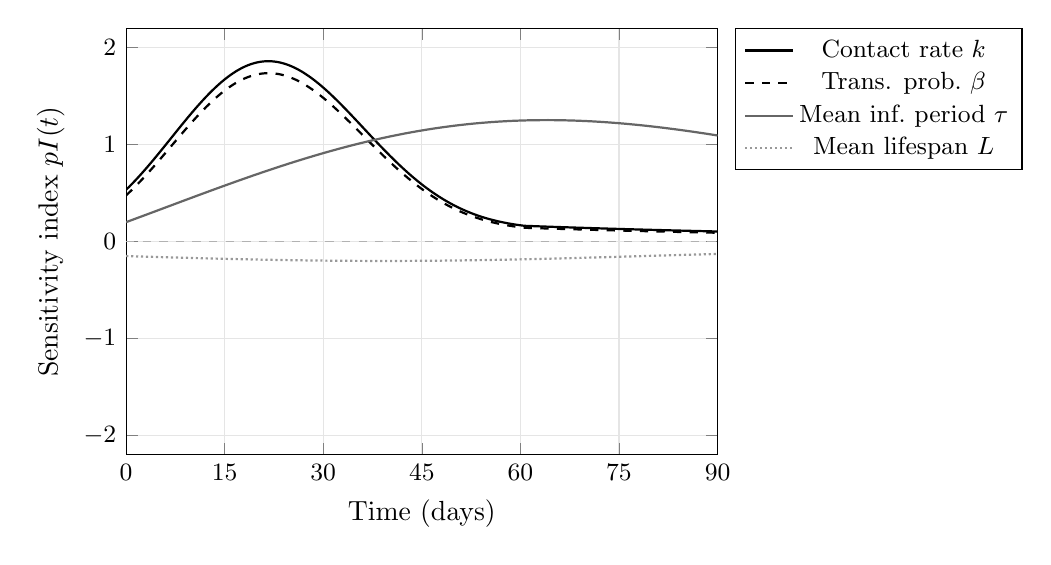
\begin{tikzpicture}
  \begin{axis}[
    width=0.75\textwidth, height=7cm,
    xlabel={Time (days)},
    ylabel={Sensitivity index $\SI{p}{I}(t)$},
    xmin=0, xmax=90,
    ymin=-2.2, ymax=2.2,
    grid=major, grid style={gray!20},
    legend pos=outer north east,
    legend style={font=\small},
    xtick={0,15,30,45,60,75,90},
    yticklabel style={font=\small},
    xticklabel style={font=\small},
  ]
  %% Schematic curves -- representative shapes based on SIR dynamics
  %% k: positive, peaks early ~day 15, then declines
  \addplot[thick, black, domain=0:90, samples=200]
    {1.8*exp(-0.04*(x-15)^2/30)*max(0.01,sin(deg(0.05*x+0.1)))
     + 0.4*exp(-0.015*x)};
  \addlegendentry{Contact rate $k$}

  %% beta: same shape as k (SI_k = SI_beta for R0 = kbeta/gamma)
  \addplot[thick, black, dashed, domain=0:90, samples=200]
    {1.7*exp(-0.04*(x-15)^2/30)*max(0.01,sin(deg(0.05*x+0.1)))
     + 0.35*exp(-0.015*x)};
  \addlegendentry{Trans. prob.\ $\beta$}

  %% tau: positive, grows after ~day 20, peaks ~day 40
  \addplot[thick, black!60, domain=0:90, samples=200]
    {0.2 + 1.4*(1-exp(-0.025*x))*exp(-0.01*(x-45)^2/60)};
  \addlegendentry{Mean inf.\ period $\tau$}

  %% L (lifespan): small negative throughout
  \addplot[thick, black!40, densely dotted, domain=0:90, samples=200]
    {-0.15 - 0.05*sin(deg(0.04*x))};
  \addlegendentry{Mean lifespan $L$}

  \draw[dashed, black!30] (axis cs:0,0) -- (axis cs:90,0);
  \end{axis}
  \end{tikzpicture}
  \caption{Schematic of time-dependent sensitivity indices $\SI{p}{I}(t)$
           for the SIR model. In the early outbreak phase, the contact
           rate $k$ and transmission probability $\beta$ (nearly equal
           because $\SI{k}{R_0} = \SI{\beta}{R_0}$) dominate.
           The mean infectious period $\tau$ grows in importance
           as the outbreak progresses. The mean lifespan $L$ has
           a small negative influence throughout. Curve shapes are
           representative; the MATLAB laboratory (Section~\ref{sec:ch4matlab})
           and the function \texttt{plot\_time\_si.m} in the companion
           repository produce exact computed curves at the nominal parameters.}
  \label{fig:sir_timevarySI}
\end{figure}

%%------------------------------------------------------------
\section{The Proliferation Problem\index{proliferation problem} and Its Consequences}
\label{sec:proliferation}
%%------------------------------------------------------------

\begin{quote}
\textit{Before improving the model, find out which knob actually moves the machine.}
\end{quote}

\medskip\noindent
The FSE is exact and efficient for a single parameter.
For $m$ parameters, the cost scales linearly: $m$ augmented ODE
solves, each requiring $n$ additional state variables.
Table~\ref{tab:prolif} quantifies this for representative models.

\medskip\noindent
\textit{Counting convention.} Throughout this section, ``solve counts''
refer to the total number of ODE solves, including the one baseline
forward solve (of the original $n$-equation system) required before
any sensitivity computation begins. The FSE adds $m$ augmented solves
on top of this baseline, for a total of $m + 1$ solves.

\begin{table}[htb]
\centering
\begin{tabular}{lrrrr}
\toprule
Model & $n$ states & $m$ \POIs & Augmented size & FSE cost \\
\midrule
SIR          & 3  & 4  & $3 + 12 = 15$  & 4 ODE solves \\
SEIR         & 4  & 6  & $4 + 24 = 28$  & 6 ODE solves \\
Malaria model & 7  & 17 & $7 + 119 = 126$ & 17 ODE solves \\
Climate model & 500 & 200 & $500 + 100{,}000$ & 200 ODE solves \\
\bottomrule
\end{tabular}
\caption{Augmented system size and FSE cost for representative models.
         For the climate model, 200 ODE solves each taking 6~hours
         equals 50 days of computation. This is the cost that
         motivates the adjoint method in Chapter~6.}
\label{tab:prolif}
\end{table}

For the SIR model, 4~solves is extremely fast in practice.
For the climate model, 200~solves at 6~hours each is 50~days.
This is the computational wall that motivates the adjoint approach.

\unifyingidea{2} Table~\ref{tab:prolif} reveals the bottleneck
that Chapters~5 and 6 resolve.
No matter how the sensitivity Jacobian is computed, by
finite differences, by analytic FSE, or by the adjoint;
the answer is the same matrix of normalized derivatives.
The adjoint (Unifying Idea~2, introduced in Chapter~5) reduces
the cost from $m$~solves to 2~solves by exploiting the
transposed structure of the problem. The cost reduction is
proportional to $m$; for $m = 200$, the adjoint is
100~times faster than the FSE.

\unifyingidea{3} Every row of Table~\ref{tab:prolif} is a linearization.
The FSE computes the exact derivative of a nonlinear model, which
is a linear approximation to the model's response. That approximation
is valid when parameters are near their nominal values. The proliferation
problem scales with $m$; the validity limitation is independent of $m$.
Chapter~8 addresses the second problem; Chapters~5 and 6 address the first.

\begin{selfcheck}
For the malaria model with $n = 7$ state variables and $m = 17$
\POIs, and one response functional (say, the endemic equilibrium
fraction $i_h$):
(a) How many ODE solves does the FSE approach require?
(b) If each ODE solve takes 2~minutes, how long does the
    complete FSA take?
(c) How many ODE solves will the adjoint method in Chapter~6 require?
\end{selfcheck}
\begin{scAnswer}
(a) 17 FSE solves (one per parameter), plus 1 forward solve = 18 total.
(b) $18 \times 2 = 36$ minutes.
(c) The adjoint always requires exactly 2 solves (1 forward + 1 adjoint),
regardless of $m$.
For 17 parameters, the adjoint is 9 times faster than the FSE.
\end{scAnswer}

%%------------------------------------------------------------
\section{The Decision Table: When to Use Which Method}
\label{sec:decisiontable}
%%------------------------------------------------------------

With three computational methods now available (finite differences,
analytic FSE, and the adjoint previewed above), the right choice
depends on the model and the problem.

\begin{table}[htb]
\centering
\renewcommand{\arraystretch}{1.3}
\begin{tabular}{p{3.2cm}p{2.8cm}p{1.5cm}p{2.8cm}p{1.2cm}}
\toprule
Situation & Method & Accuracy & Cost & When to use \\
\midrule
Black-box model & Finite differences & $O(h^2)$ & $2n_p + 1$ evals & Ch 3 \\
Analytic, small $n_p$ & FSE & Exact & $n_p$ solves & Ch 4 \\
Analytic, large $n_p$ & Adjoint & Exact & 2 solves & Ch 5--6 \\
Correlated \POIs & Reparameterize first & --- & --- & Ch 3 \\
Model near bifurcation & FSE + caution & Exact* & $n_p$ solves & Ch 8 \\
Large parameter uncertainty & Global SA & Variance-based & $N(m+2)$ evals & Ch 9 \\
\bottomrule
\end{tabular}
\caption{Decision table for selecting the SA computational method.
         For a systematic benchmarking of these methods on biological ODE
         models, see Mester et al.~\cite{mester2022differential}.
         (*Near a bifurcation, the FSE solution is exact but the
         sensitivity index diverges, limiting its interpretability.)}
\label{tab:decision}
\end{table}

For this course, the default progression is:
\begin{enumerate}[nosep]
  \item Start with finite differences (Chapter~3) to get SA results quickly.
  \item Switch to analytic FSE (this chapter) when the model is differentiable
        and accuracy matters.
  \item Use the adjoint (Chapters~5--6) when $m$ is large.
  \item Check for correlated \POIs before reporting any results (Chapter~3).
  \item Consider global SA (Chapter~9) when parameter uncertainty is large.
\end{enumerate}

A common assumption is that finite differences are adequate for
any SA study once the step size is chosen correctly.
For black-box models, this is true: FD is the only option
and produces reliable results at the optimal step size.
For differentiable models, the analytic FSE is
simultaneously more accurate (exact rather than $O(h^2)$)
and often faster (no repeated model evaluations at perturbed
parameter values). The two methods give the same numbers
when FD is implemented correctly; the FSE gives those same
numbers without approximation error and without the
step-size selection problem.

%%------------------------------------------------------------
\section{MATLAB Laboratory: Analytic FSA of the SIR Model}
\label{sec:ch4matlab}
%%------------------------------------------------------------

This laboratory implements the augmented ODE system for the SIR model
and compares the analytic FSE approach with the finite-difference
method from Chapter~3.

\textbf{Setup.}
Use the SIR model~\eqref{eq:sirS}--\eqref{eq:sirR} with
\POIs $\vec{p} = (k, \beta, \tau, L)$ (interpretable parameterization),
nominal values $k = 5$, $\beta = 0.06$, $\tau = 7$~days, $L = 10{,}000$~days,
and initial conditions $S_0 = 999$, $I_0 = 1$, $R_0 = 0$, $N = 1000$.

\textbf{Part 1:} Implement the augmented ODE system.
Write a MATLAB function \texttt{sir\_augmented(t, y, k, beta, tau, L)}
that returns the derivatives for the full $15$-equation augmented system:
3~original state equations plus $4 \times 3 = 12$ FSE equations.
The FSE equations require the Jacobian of $(F_S, F_I, F_R)$ with
respect to $(S, I, R)$.

\medskip\noindent
\textit{State vector layout.} The 15-component state vector \texttt{y}
is organized as follows:
\begin{center}
\begin{tabular}{cl}
\toprule
Index & Meaning \\
\midrule
1 & $S(t)$ \\
2 & $I(t)$ \\
3 & $R(t)$ \\
4--6   & $(\partial S/\partial k,\; \partial I/\partial k,\; \partial R/\partial k)$ \\
7--9   & $(\partial S/\partial\beta,\; \partial I/\partial\beta,\; \partial R/\partial\beta)$ \\
10--12 & $(\partial S/\partial\tau,\; \partial I/\partial\tau,\; \partial R/\partial\tau)$ \\
13--15 & $(\partial S/\partial L,\; \partial I/\partial L,\; \partial R/\partial L)$ \\
\bottomrule
\end{tabular}
\end{center}
The initial condition is \texttt{y0 = [S0; I0; 0; zeros(12,1)]}.
The sensitivity variables all start at zero because the initial
conditions do not depend on the parameters.
The file \texttt{sir\_augmented.m} in the companion repository
implements this system and may be used as a reference after
completing your own implementation.

\textbf{Part 2:} Solve and extract sensitivities.
Solve the augmented system from $t = 0$ to $t = 90$~days
using \texttt{ode45}. Extract the time-dependent sensitivity indices
$\SI{k}{I}(t)$, $\SI{\beta}{I}(t)$, $\SI{\tau}{I}(t)$, $\SI{L}{I}(t)$.

\textbf{Part 3:} Plot time-dependent SIs.
Plot all four $\SI{p_j}{I}(t)$ curves on a single axis, alongside the
epidemic curve $I(t)$. Identify:
(a) at $t = 10$~days, which parameter matters most?
(b) at $t = 50$~days, has the ranking changed?
(c) which parameter has the largest absolute SI at the epidemic peak?

\textbf{Part 4:} Compare with finite differences.
At $t = 30$~days and $t = 70$~days, compare the FSE-based SI values
against the centered-difference estimates from Chapter~3.
Are they equal to 4~significant figures? Report any discrepancies
and explain their likely source.

\textbf{Part 5:} Cost comparison.
Time the two approaches: the augmented ODE (all 4 sensitivities at once)
versus 4 separate centered-difference calls to \texttt{SIR\_model}.
Which is faster? Which is more accurate? At what value of $m$
(number of \POIs) would you expect the two approaches to take
approximately equal time?

%%------------------------------------------------------------
\section{Exercises}
\label{sec:ch4exercises}
%%------------------------------------------------------------

\begin{exercise}[\bloom{L2}]
\label{ex:ch4:pattern}
State the three-step FSE derivation pattern in your own words,
without using any symbols. Then explain, in one sentence, why
the FSE is always linear in the sensitivity variable even when
the original equation is nonlinear.
\end{exercise}

\begin{exercise}[\bloom{L3}]
\label{ex:ch4:implicit}
For the nonlinear equation $g(u; p) := u^3 - 3pu + 2 = 0$:
\begin{enumerate}[label=(\alph*)]
  \item Write the FSE for $\partial u/\partial p$.
  \item At $p = 1$, find all real roots $u$ numerically.
  \item Compute $\SI{p}{u}$ at each root.
  \item At $p = 1$, for which root is the sensitivity largest in magnitude?
        Verify your answer using a centered finite difference with optimal $h$.
\end{enumerate}
\end{exercise}

\begin{exercise}[\bloom{L3}]
\label{ex:ch4:logistic}
For the logistic ODE $\dot{u} = ru(1-u/K)$, $u(0) = u_0$:
\begin{enumerate}[label=(\alph*)]
  \item Write the FSE for $w_r = \partial u/\partial r$.
  \item Verify that the FSE is linear in $w_r$ by identifying
        the coefficient (which depends on $u(t)$) and the forcing term.
  \item Using MATLAB, implement the augmented system
        $(u, w_r, w_K)$ and solve from $t = 0$ to $t = 20$.
  \item Plot $\SI{r}{u}(t)$ and $\SI{K}{u}(t)$.
        Interpret: near $t = 0$ vs.\ near the carrying capacity.
\end{enumerate}
\end{exercise}

\begin{exercise}[\bloom{L3}]
\label{ex:ch4:symbiotic}
For the symbiotic population model~\eqref{eq:symp1}--\eqref{eq:symp2}
with $a = 0.5$, $b = 2$, $c = 0.4$:
\begin{enumerate}[label=(\alph*)]
  \item Compute the coexistence equilibrium.
  \item Assemble and solve the FSE for $\partial\vec{u}/\partial c$.
  \item Compute the normalized sensitivity indices
        $\SI{c}{\bar{u}_1}$ and $\SI{c}{\bar{u}_2}$.
  \item Using equation~\eqref{eq:sympeq}, compute the same indices
        analytically. Verify agreement.
\end{enumerate}
\end{exercise}

\begin{exercise}[\bloom{L4}]
\label{ex:ch4:proliferation}
The SEIRS model (Susceptible-Exposed-Infectious-Recovered-Susceptible)
has 4 state variables and 7 parameters.
\begin{enumerate}[label=(\alph*)]
  \item How many ODEs are in the augmented FSE system for all 7 parameters?
  \item If each ODE solve takes 3~minutes, how long does the full FSA take
        using the FSE approach? The adjoint approach (Chapter~6)?
  \item Suppose a modeler decides to reduce computation time by computing
        sensitivities only for the 3 parameters they expect to be most
        important, based on biological intuition. Identify one scenario
        where this strategy would lead to a misleading conclusion.
\end{enumerate}
\end{exercise}

\begin{exercise}[\bloom{L4}]
\label{ex:ch4:sirtime}
Using your MATLAB implementation from the laboratory:
\begin{enumerate}[label=(\alph*)]
  \item At three time points, $t = 5$ (early epidemic),
        $t = t_{\text{peak}}$ (peak infections), and $t = 80$ (late);
        report the tornado plot of SIs for $I(t)$.
  \item Does the parameter ranking change across the three time points?
  \item A public health officer says: ``We should target the parameter
        with the largest SI at the epidemic peak, since that is when the
        most people are affected.'' Critique this statement using your results.
\end{enumerate}
\end{exercise}

\begin{exercise}[\bloom{L5}]
\label{ex:ch4:design}
A colleague is modeling cholera transmission with a SEIR-type model
having 8 parameters and 4 state variables.
She asks for advice on the SA methodology.
Design a complete FSA study, specifying:
\begin{enumerate}[label=(\alph*)]
  \item Whether to use finite differences or analytic FSE, and why.
  \item How you would validate the implementation.
  \item What \QOIs you would compute sensitivity indices for,
        and at what time points.
  \item How you would present the results to identify the
        two most critical intervention targets.
  \item One situation in which the FSE results might be misleading,
        and what additional analysis you would recommend.
\end{enumerate}
\end{exercise}

\begin{exercise}[\bloom{L6}]
\label{ex:ch4:critique}
A published paper reports: ``We performed sensitivity analysis of the
SEIR model using the forward sensitivity equations. All sensitivity
indices were computed at $t = 365$~days, giving a single set of
values for the entire epidemic.''

The model simulates a disease whose outbreak dynamics play out
over approximately 60~days, but the model runs for a year.

Identify at least two methodological issues with this approach.
For each issue, state what the authors should have done instead
and explain what information they likely missed.
\end{exercise}

%%------------------------------------------------------------

